\newpage
\section{Ansible}

Ansible es una herramienta idempotente \textbf{asegura el mismo resultado siempre}. Que permite orquestar y configurar desde un simple servidor hasta un datacenter completo, todo realizado a través de SSH que permite que podamos ejecutar las instrucciones
u obtener información de monitoreo básica de manera segura.

\subsection{Instalación de Ansible en Debian/Ubuntu}

Primero necesitamos instalar los repositorios de Ansible antes de proceder a su instalación. Para ello ejecutamos los siguientes comandos:
\begin{lstlisting}[style=mybash]
$ echo "deb http://ppa.launchpad.net/ansible/ansible/ubuntu focal main" | sudo tee /etc/apt/sources.list.d/ansible.list
$ sudo apt-key adv --keyserver keyserver.ubuntu.com --recv-keys 93C4A3FD7BB9C367
$ sudo apt update
$ sudo apt install ansible
\end{lstlisting}

Ejecutando los comandos de arriba obtendremos lo siguiente:

\begin{figure}[H]
	\centering
	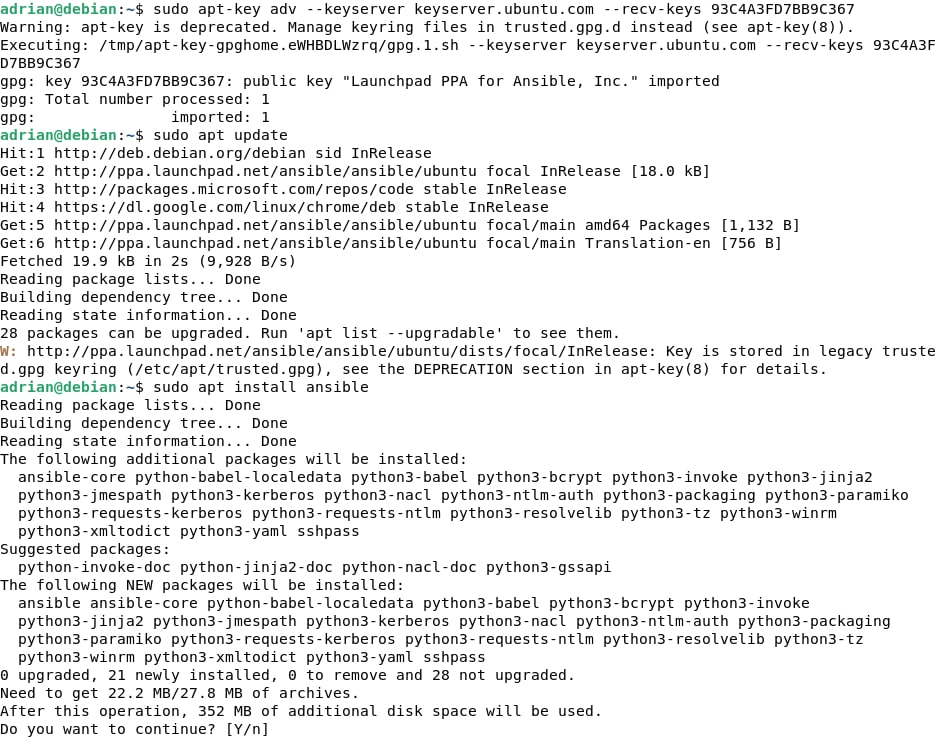
\includegraphics[scale=0.35]{img/ansible0}
	\caption{Instalación de Ansible.}
\end{figure}

\newpage
\subsection{Inventario}

El entorno a controlar se puede definir en un fichero llamado \textbf{inventory.yml} que indicamos en el las direcciones IP y los hostname para identificar a cada servidor particular. Así como crear grupos con los cuales podemos usar como objetivo de determinadas tareas.

En el proyecto usamos 3 tipos de grupos:
webservers, loadbalancer y databases.

Esto nos permite lanzar a todas las direcciones de los contenedores, máquinas virtuales, servidores físicos (on-prem), etc...

Así como podemos agrupar los grupos con hostnames y direcciones en otros grupos padre simbólicoss. Esto es útil en el caso de que necesitemos agruparlos para usar Playbooks que resuelvan necesidades específicas como por ejemplo: Realizar copias de seguridad de /var/log/nginx, para almacenar los logs de manera segura para tener un análisis del tráfico de los balanceadores y los servidores web.

\textbf{Nota:} Para que ansible pueda identificar el fichero de inventario. Necesitamos usar otro fichero llamado \textbf{ansible.cfg} en el cual tenemos que poner como parámetro el inventario que va a usarse para lanzar los Playbooks.

Fichero donde definimos el inventario a utilizar por parte de Ansible \emph{ansible.cfg}

\lstinputlisting[style=myyaml]{../ansible.cfg}

Fichero de inventarios. \emph{inventory.yml}

\lstinputlisting[style=myyaml]{../inventory.yml}

En el fichero definimos desde la raíz del árbol de grupos hasta los hostnames como sigue:

\begin{itemize}
    \item \textbf{datacenter} - Grupo padre de todos que apunta a todos los subgrupos del inventario. Útil para tareas de monitorización y comprobación de estados con un simple ping ejecutado desde comandos de Ansible Ad-hoc.
    \begin{itemize}
        \item \textbf{datacenterweb} - Sub-Grupo hijo de datacenter que tiene de hijos solo a los sub-grubpos webservers y loadbalancers.
        \begin{itemize}
            \item \textbf{webservers} - Sub-Grupo hijo de datacenterweb que apunta a los hostnames y direcciones IPs de los servidores web indexados con Ansible.
            \item \textbf{loadbalacer} - Sub-Grupo hijo de datacenterweb que apunta a los hostnames y direcciones IPs de los balanceadores de carga web indexados con Ansible.
        \end{itemize}
        \item \textbf{databases} - Sub-Grupo hijo de datacenter que apunta a los hostnames y direcciones IPs de los servidores SGBD.
    \end{itemize}
\end{itemize}

\subsection{Ansible-playbooks}

Los Playbooks son archivos de \emph{orquestación} que nos permiten modularizar el aprovisionamiento y ejecución.

La estructura del Playbook empieza con la definición del grupo, o a un hostname concreto (un servidor) al que afecta las tareas ejecutadas y a continuación se define variables o no.

Lo importante del Playbook, es que podemos definir un Playbook de tal manera que nos permita realizar un objetivo final concreto que requiere de un sin número de pasos, o tareas, como desplegar una base de datos y asegurarla. Pues en una terminal sería como sigue:

\begin{lstlisting}[style=mybash]
$ sudo apt-get install mariadb-server -y
$ sudo systemctl enable mariadb-server.service
$ sudo systemctl start mariadb-server.service
$ sudo mysql_secure_installation
\end{lstlisting}

\emph{¿Podemos automatizarlo con un script?} Sí, pero si ocurren casos como que, mariadb esté instalado o el servicio no se ejecute bien en un sistema en concreto, el script dejaría de funcionar o necesitamos destinar recursos para programar una ejecución de errores
que sería muy concreto y poco portable a otras plataformas.

\vspace{5mm}

Además de que tendríamos que diseñar el script para apuntar a los servidores o máquinas concretas, complicando el diseño ya que necesitaremos una estructura de datos concreta que permita indexar los hostnames, servidores y control de errores. Entonces si tenemos 40 servidores web, nos encontramos que en caso de fallo, esos servidores podrían quedarse inutilizados.
O que la instalación prosiga pero en un estado erroneo sin informarnos debidamente.

\vspace{5mm}

Todo eso se soluciona con un Playbook que funciona de manera idempotente y que con solo pequeños cambios podemos reutilizarlo para otra distribución Red Hat style o Debian style ...

Veremos el caso de Mariadb en la siguiente subseccion

\subsection{Playbooks usados para el proyecto y para qué sirven.}

\subsubsection{Playbook de hosts.yml}

Este Playbook ha sido diseñado de tal manera que será el padre de todos los playbook a los que va llamando sucesivamente. Pero podemos comentar las lineas de import\_playbook para que solo se ejecute simplemente el proposito de \emph{hosts.yml}.

Su propósito es el de a partir de la pantilla localizada en \textbf{templates/hosts.j2}. Que contiene lo siguiente:

\lstinputlisting[style=myyaml]{../templates/hosts.j2}
\vspace{5mm}

En el template podemos ver que se genera una línea de host por cada variable encontrada (demoninado también Facts de Ansible) en el fihero inventory.yml de Ansible que ejecuta el Playbook. Lo cual es muy últil para obtener de manera dinámica todos los hostnames asociados a su dirección IP sin tener que realizar el proceso manual de añadir un servidor nuevo a mano a cada fichero hosts. Si no tenemos un DNS.
\vspace{5mm}

Se puede comentar las lineas de incluir otros Playbook. Permitiendo que se ejecute de manera individual la tarea, para generar ficheros de hosts en el caso de que se añada al inventario muchos mas servidores. Con ello nos aseguramos de que cada servidor va a tener su fichero hosts siempre actualizado.

\lstinputlisting[style=myyaml]{../playbooks/hosts.yml}

\begin{figure}[H]
	\centering
	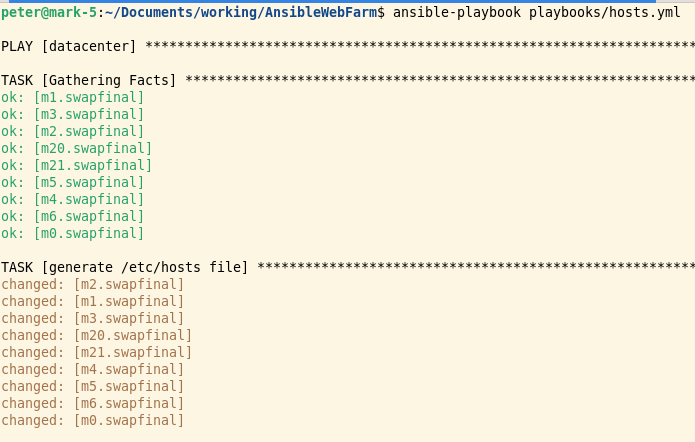
\includegraphics[scale=0.35]{img/ansible1}
	\caption{Generación de los ficheros /etc/hosts en el Playbook.}
\end{figure}

El funcionamiento básico del playbook es:

\begin{itemize}
	\item Sección \textbf{PLAY [datacenter]}: Indica en qué grupos del inventario se está aplicando el Playbook. En este caso se aplica para todo el mundo ya que datacenter es el grupo padre de todos los grupos.
	\item Sección \textbf{TASK [Gathering Facts]}: Es la sección donde Ansible asegura que los hosts referenciados están disponibles, si falla uno no aplica el Playbook. Ya que debe ser idempotente, es decir que se aplica a todo o a nada.
	\item Sección \textbf{TASK [generate /etc/hosts file]}: Es la tarea en la que se especializa el Playbook que genera a partir de la plantilla y lo lleva a todo el grupo llamado datacenter. El estado de changed indica que se ha aplicado los cambios de manera correcta.
\end{itemize}

\begin{figure}[H]
	\centering
	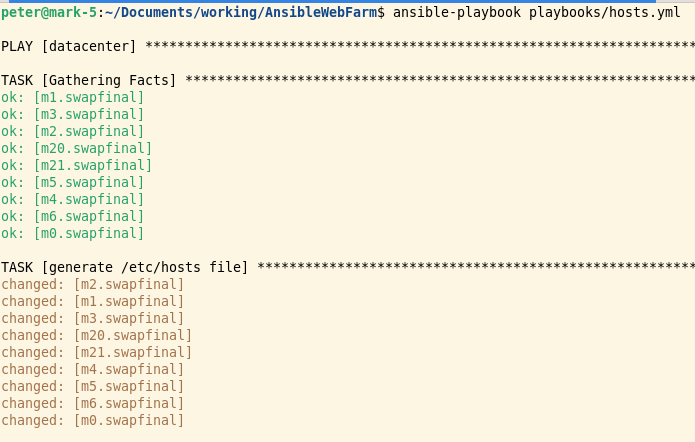
\includegraphics[scale=0.35]{img/ansible1}
	\caption{Generación de los ficheros /etc/hosts en el Playbook.}
\end{figure}

\begin{figure}[H]
	\centering
	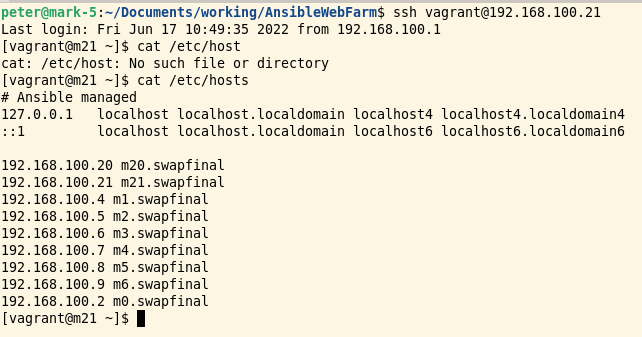
\includegraphics[scale=0.35]{img/ansible2}
	\caption{Ficheros de /etc/hosts generados en los servidores de base de datos como ejemplo, en este caso es m20-swapfinal.}
\end{figure}

\newpage
\subsubsection{Playbook de SSL.yml}

Este Playbook puede parecer muy largo pero es sencillo. Necesita la colección de \textbf{community.crypto}. Que es una serie de colecciones que nos permite realizar determinadas acciones que no se hacen de manera nativa en Ansible. Si no que son extendidas por la propia comunidad de usuarios.
\vspace{5mm}

Esta colección nos permite realizar muchas opciones desde generar una CA hasta un certificado X.509, con Ansible. Pudiendo como en mi caso hacer un Playbook que especificando una serie de tareas, podemos replicar todo el proceso necesario para generar una clave, generar un CSR Certificate Signed Request, generar el Certificado Firmado. A su vez incluir la firma de la CA y incluir su Certificado para validar el certificado del dominio.
\vspace{5mm}

Para instalar la colección necesitamos ejecutar lo siguiente:

\begin{lstlisting}[style=mybash]
	# Instalacion de la coleccion de crypto para crear CA
	$ ansible-galaxy collection install community.crypto
\end{lstlisting}

\textbf{Nota:} Todo este proceso lo realizamos en un balanceador en concreto, en mi caso es m0-swapfinal. Esto es debido a que no necesitamos generar N claves y certificados, si lo ejecutamos en un grupo en concreto como loadbalancer o webservers. Entonces lo que hacemos es especificar el hostname de un balanceador de carga que va a asumir el proceso entero.

\begin{itemize}
	\item La primera parte es que instala las dependencias necesarias para que Ansible pueda trabajar con la colección ya que usa paquetes de Python. En concreto el paquete cryptography.
	\item La segunda parte son todas las tareas que se requieren para generar una CA y sus certificados.
	\item La tercera parte son todas las tareas que se requieren para generar el certificado de swapfinal y firmarlo con la CA.
	\item La cuarta parte es el proceso de copia de todos los ficheros CRT y KEY menos el de la CA.key. Al ordenador del administrador.
	\item La última parte es la ejecución de otro Playbook que permite la copia de los certificados y claves copiados a cada uno de los servidores web. Que son necesarios para poder configurar su HTTPs.
\end{itemize}

\begin{figure}[H]
	\centering
	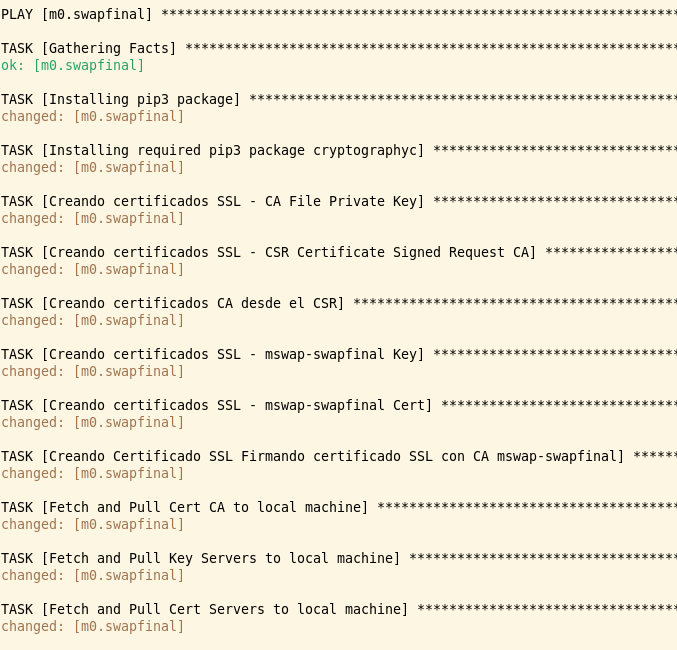
\includegraphics[scale=0.35]{ansible3}
	\caption{Ejecución de la parte de creación de los certificados SSL y claves de CA y swapfinal.}
\end{figure}

Ahora podemos ver el proceso de copiado de las claves y certificados necesarios para los servidores web. Se puede ver que la sección \textbf{PLAY [webservers]}. Indica que se está ejecutando en el grupo perteneciente a los servidores web.

\begin{figure}[H]
	\centering
	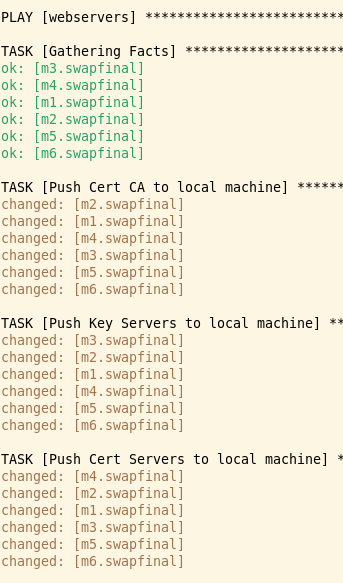
\includegraphics[scale=0.35]{ansible4}
	\caption{Ejecución de la parte de copiado de los certificados y claves necesarias para los servidores web.}
\end{figure}

\begin{figure}[H]
	\centering
	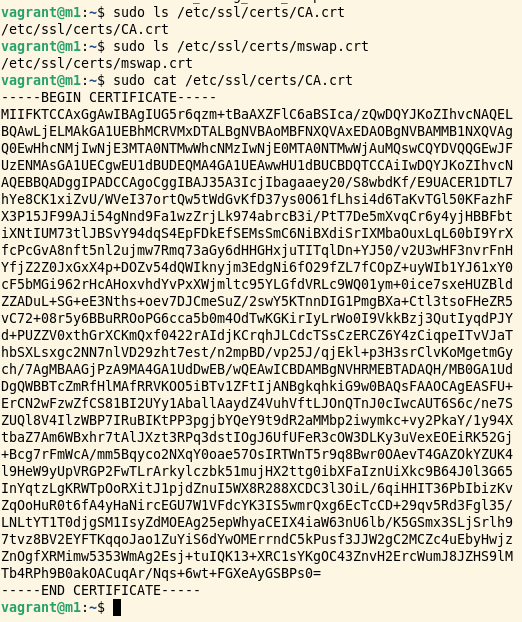
\includegraphics[scale=0.35]{ansible5}
	\caption{Ficheros correctamente copiados.}
\end{figure}

\newpage
\subsubsection{Playbook de webservers.yml}

Este playbook tiene varios objetivos:

\begin{itemize}
	\item La primera parte es instalar Nginx, PHP y PHP-fpm necesario para ofrecer una web más dinámica que ofrezca una vista de lo que ocurre cuando solicites el index.php al balanceador.
	\item La segunda parte es el proceso de copia del fichero de configuración del sitio por defecto. Que debemos definir como plantilla, para exportarla y aplicarla a todos los servidores.
	\item La tercera parte es el proceso de copia del index.php base de plantilla, que debe ser llevado a todos los servidores. A /var/www/html/.
	\item La cuarta parte una vez terminado el proceso de copia anterior, reiniciamos, el servicio para que aplique los cambios del sitio por defecto y que arranque PHP. Además de fijarlo como si ejecutamos \textbf{sudo systemctl enable nginx.service}. Para que en cada reinicio siempre esté activado.
\end{itemize}

El playbook en cuestión es el siguiente:

\lstinputlisting[style=myyaml]{../playbooks/webservers.yml}

Para los ficheros de index.php tenemos una lectura de la variable de \textbf{\$\_SERVER['SERVER\_ADDR']}. Que como se ha especificado antes nos permite identificar que se hagan peticiones en Round Robin con weight 1 a los servidores web.

\lstinputlisting[style=myhtml]{../templates/index.php}

\begin{figure}[H]
	\centering
	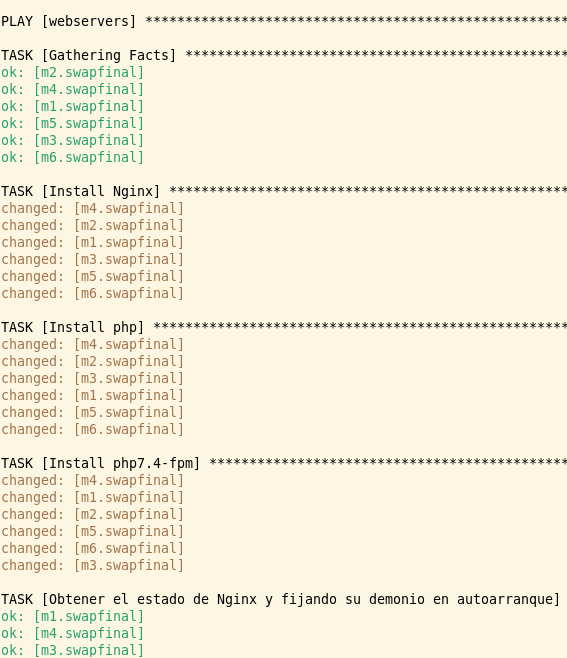
\includegraphics[scale=0.35]{ansible6}
	\caption{Proceso de ejecución del playbook webservers.yml}
\end{figure}

\begin{figure}[H]
	\centering
	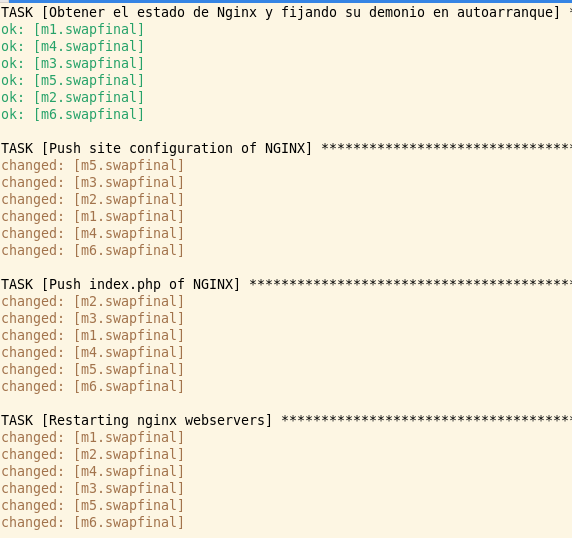
\includegraphics[scale=0.35]{ansible7}
	\caption{Proceso de ejecución del playbook webservers.yml, segunda parte consistente en fijar el demonio, configurarlo y fijar sus . }
\end{figure}

\begin{figure}[H]
	\centering
	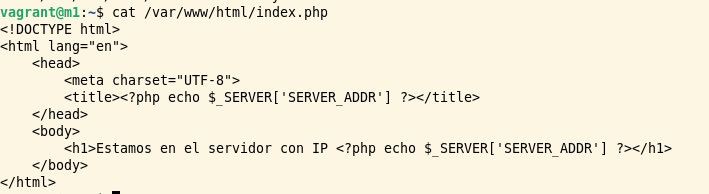
\includegraphics[scale=0.35]{ansible8}
	\caption{Fichero index.php correctamente copiado.}
\end{figure}

\newpage
\subsubsection{Playbook de loadbalancer.yml}

\textbf{Recordemos:} Se está utilizando NGINX como balanceador de carga.

Este playbook tiene varios objetivos:

\begin{itemize}
	\item La primera parte es instalar Nginx y preparando el autoarranque del demonio de Nginx.
	\item La segunda parte la desactivación de la web por defecto que incluye. Usando un comando de bash sencillo a través de Ansible y que además nos asegura la correcta ejecución de este.
	\item La tercera parte es la generación del template del fichero de configuración del balanceador de carga. Esto es debido a que hay un número variable de servidores web, nos encontramos con que necesitamos el template .j2 que nos permita indicar en la parte de upstream los servidores web a los que debe hacer de balanceador de carga con el indicador del grupo de webservers.
	\item La cuarta parte una vez terminado el proceso de copia anterior, reiniciamos, el servicio para que aplique los cambios al balanceador.
\end{itemize}

\textbf{El playbook del balanceador es el siguiente:}
\vspace{5mm}
\lstinputlisting[style=myyaml]{../playbooks/loadbalancer.yml}
\vspace{5mm}

\textbf{El template del fichero de configuración del balanceador es el siguiente:}
\vspace{5mm}
\lstinputlisting[style=myyaml]{../templates/lbnginx.j2}
\vspace{5mm}

La parte variable es un bucle sencillo similar al de la plantilla de hosts. Pero con la particularidad de que apuntamos a un grupo distinto al que ejecuta el playbook (webservers).

\begin{figure}[H]
	\centering
	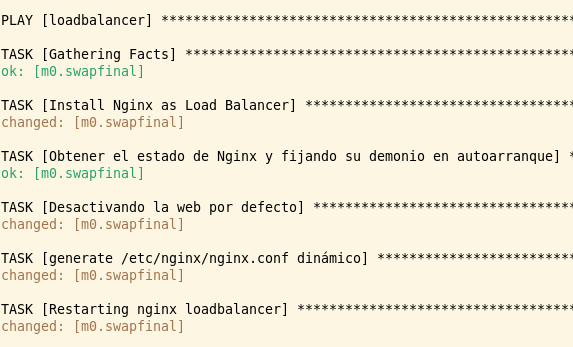
\includegraphics[scale=0.35]{ansible9}
	\caption{Ejecución del PlayBook de loadbalancer.}
\end{figure}

\begin{figure}[H]
	\centering
	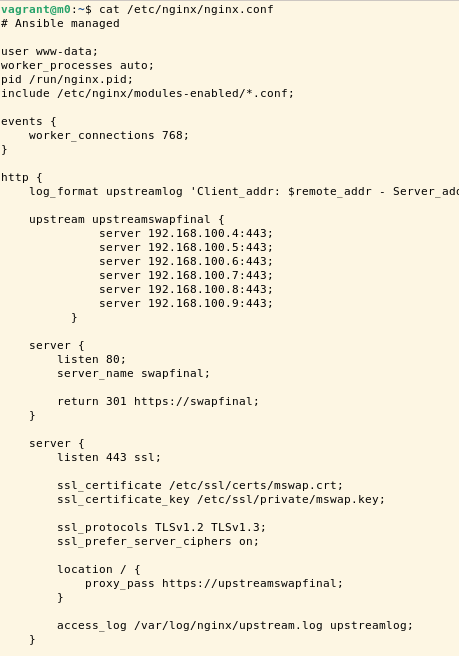
\includegraphics[scale=0.35]{ansible10}
	\caption{Fichero de configuración generado solo con los webservers.}
\end{figure}

\newpage
\subsubsection{Playbook de databases.yml}

Este playbook tiene varios objetivos:

\begin{itemize}
	\item La primera parte es instalar Mariadb como SGBD.
	\item La segunda parte es introducir un .my.cnf que incluye una clave por defecto para que permita en el usuario vagrant que es el que se usa para conectarse con Ansible y Vagrant. El acceso root de mysql.
	\item La tercera parte es añadir PyMySQL que es el driver que permite las conexiones con el SGBD a través de Python que es necesario para ejecutar la collection de community.MySQL.
	\item La cuarta parte es el proceso de mysql\_secure\_installation imitado en un Ansible Playbook, porque el original es un script de bash interactivo. Entonces aquí hacemos todo el proceso integrado con Ansible para que se ejecute en los N servidores SGBD.
\end{itemize}

Para instalar la colección de Mysql necesaria para realizar el proceso.

\begin{lstlisting}[style=mybash]
	# Instalacion de la coleccion de crypto para crear CA
	$ ansible-galaxy collection install community.mysql
\end{lstlisting}

\textbf{El playbook de los SGBD es el siguiente:}
\vspace{5mm}
\lstinputlisting[style=myyaml]{../playbooks/loadbalancer.yml}
\vspace{5mm}

\textbf{El template del fichero my.cnf:}
\vspace{5mm}
\lstinputlisting[style=myyaml]{../templates/my.cnf}
\vspace{5mm}

\begin{figure}[H]
	\centering
	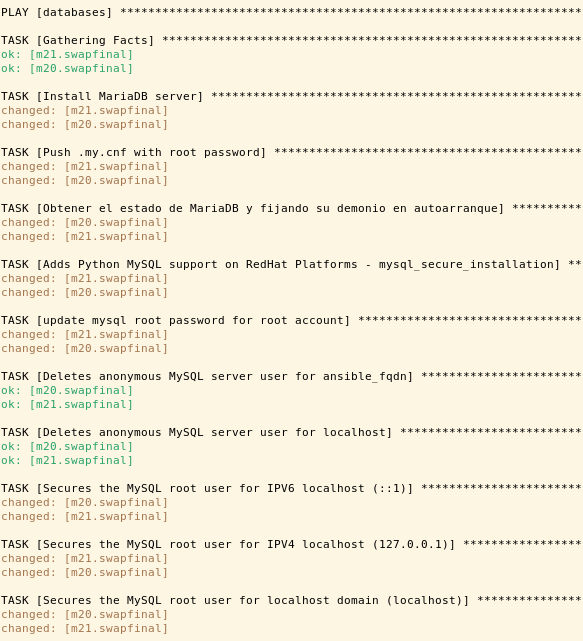
\includegraphics[scale=0.35]{ansible11}
	\caption{Proceso de instalación del SGBD y mysql\_secure\_installation.}
\end{figure}

\newpage
\section{Conclusiones}

Como conclusión es que Ansible es una herramienta que ha sido tan potente que nos ha simplificado el proceso de despliegue de un par de días a minutos. La única parte a tener en consideración es que no te libera de tener que montar y investigar manualmente una instalación previa. Para ir probando los ajustes que quieras tener de cara a un despliegue dinámico de la infraestructura.
\vspace{5mm}

Esto es con NGINX como ejemplo. La instalación es nativa con Ansible, pero la configuración y las plantillas relacionadas con NGINX requieren un conocimiento previo necesario. Porque de lo contrario Ansible más que ayudar solo estorbaría al no conocer el background que tiene el despliegue.

Ansible es una navaja suiza, pero antes debes conocer que hace cada parte de la navaja suiza y cómo aplicarla en según qué casos. En el caso de NGINX si hacemos la parte manual sabemos qué ficheros de configuración tocar y qué partes son variables a ajustar con plantillas con los hosts de Ansible.

En el futuro se seguirá usándola y mejorándose. En mi repositorio se publicarán las actualizaciones con Ansible. Se mejorará con Roles propios y mejor escalabilidad.

\begin{figure}[H]
	\centering
	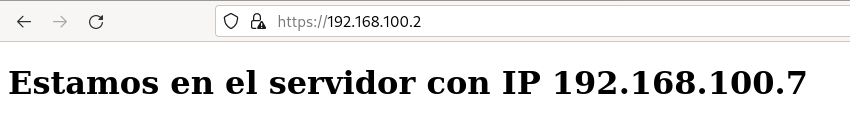
\includegraphics[scale=0.35]{ansible12}
	\caption{Balanceador en ejecución.}
\end{figure}

\begin{figure}[H]
	\centering
	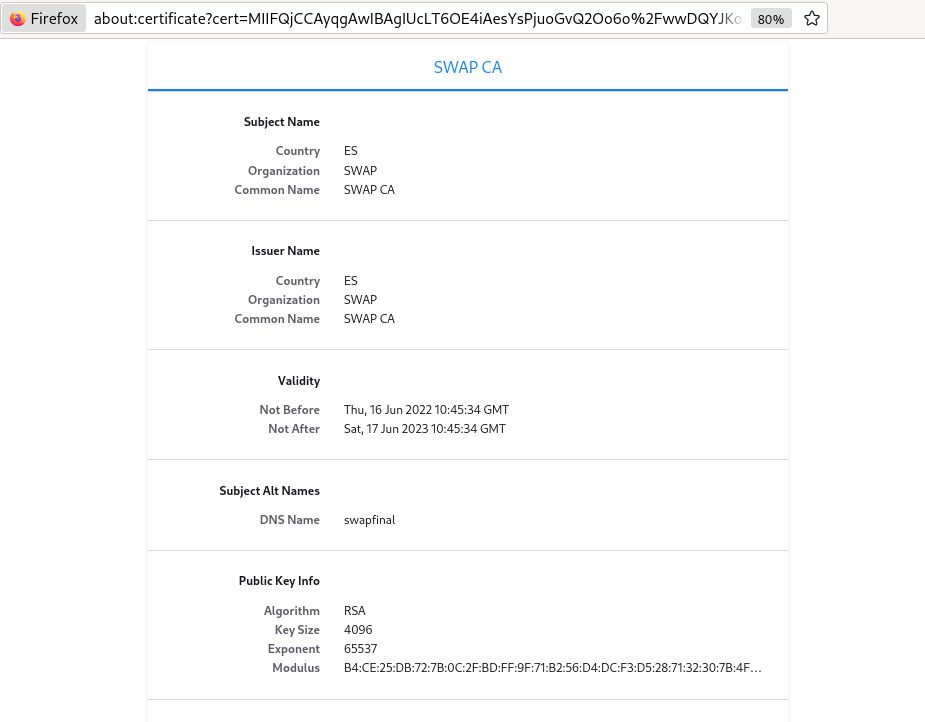
\includegraphics[scale=0.35]{ansible13}
	\caption{Certificado de swapfinal.}
\end{figure}
